\chapter{Stochastische Modelle in der Robotik}
Jede elaborierte Methoden erfordert einen Rahmen, in dem sie erarbeitet, formuliert und optimiert werden kann. In technischen Aufgabenstellung erfüllt die Mathematik diese Forderunge, weshalb die Gegebenheiten und Probleme des hiesigen Anwendungsfall zunächst in einem mathematischen Kontext dargestellt werden. Denn nur von dieser Basis ausgehend, besteht die Aussicht auf eine elegante und ansprechende Lösung.

Wie alle Probleme der Robotik, kann auch die autonome Navigation im entferntesten Sinne als Interaktion eines Roboters mit seiner Umwelt aufgefasst werden. Anhand von gesammelten Informationen muss das System eine Entscheidung über seine zukünftigen Aktionen treffen, wobei ein entferntes Ziel ohne ungewollte Kollisionen angesteuert werden soll. Für diese Aufgaben spielen drei Größen eine fundamentale Rolle. Zunächst muss die Position des Roboters beachtet werden, welche in dem Positionsvektor $\mVec{x}(t) \equiv \mVec{x}_t$ erfasst wird. Mithilfe von Sensoren sammelt der Roboter Informationen über seine Umgebung, die in dem Messvektor $\mVec{z}_t$ zusammengefasst werden. Anhand der Mess- und Positionsvektoren wird über die nächste Aktion des Roboters entschieden, die in dem Steuervektor $\mVec{u}_t$ ausgedrückt wird. Die exakte Form der Positions-, Mess- und Steuervektoren hängt von dem gegebenen Anwendungsfall und gewählten Modellformen ab, die im Folgenden näher erläutert werden.

In anderen Fachgebieten, die sich mit der Planung von Steuersignalen bzw. -sequenzen beschäftigen - wie z.B. die Regelungstechnik -, haben sich modellbasierte Methoden bewährt. Zunächst wird auf Basis von physikalischen Gegebenheiten der Zusammenhang zwischen Steuer-, Zustands- und Messvektor hergeleitet, der anschließend genutzt wird, um eine Regelstrategie zu formulieren. Der resultierende Algorithmus berechnet die Stellgröße $\mVec{u}_t$, wofür die aktuellen Mess- und Zustandsvektoren herangezogen werden. Insofern liegt es nahe modellbasierte Ansätze auch bei Problemen der Robotik zu verfolgen. Allerdings kommt dort die ungemeine Komplexität der Problemstellung zu tragen, die sich recht leicht am Beispiel der Navigation illustrieren lässt: Als erstes muss ein Modell für den Einfluss des Stellvektors $\mVec{u}_t$ auf den Positionsvektor $\mVec{x}_t$ erstellt werden. Bei mobilen Roboterplattformen handelt es sich um mechanische Systeme mit mehreren Freiheitsgraden, womit die analytische Modellbildung zwar möglich, jedoch mit einem beachtlichen Aufwand verbunden ist. Spätestens bei der Modelierung der Sensoren werden die Grenzen des Möglichen erreicht: Soll beispielsweise die Position des Roboters mithilfe von Stereokameras erfasst werden kann praktisch kaum ein exaktes, deterministisches Modell für diesen Vorgang erfasst werden, da er von zu vielen unbekannten Einflussfaktoren betroffen ist. Zuletzt kann die Pfadplanung per Definition nicht anhand eines deterministischen Modell erfolgen, da der Roboter dynamischen Hindernissen ausweichen soll, deren Form, Bewegung in der Aufgabenstellung nicht näher spezifiziert werden.

Aus diesen Gründen haben sich in der Robotik stochastische Modellformen etabliert, wobei recht simple Ausgangsmodelle verwendet werden, die um Zufallsvariablen ergänzt werden, um die Ungenauigkeiten und Ungewissheiten des Modells zu repräsentieren. Das Ziel besteht nicht mehr darin konkrete Aussagen über den Verlauf von Zustandsgrößen zu treffen, wie dies z.B. bei einer Zustandsraumdarstellung der Form
\begin{equation}
\mVec{x}(n+1) = \mat{{A}}\cdot \mVec{x}(n) + \mat{B}\cdot \mVec{\mathbf{u}}(n)
\end{equation}
erfolgt. Vielmehr soll mithilfe des Modells eine bedingte Wahrscheinlichkeit
\begin{equation}
\condP{\mVec{x}(n+1)}{\mVec{x}(n), \mVec{u}(n)}
\end{equation}
berechnet werden. Im Anschluss können die Methoden der Wahrscheinlichkeitstheorie genutzt werden, um Filter- und Planungsalgorithmen zu entwerfen. Um einen ersten Eindruck für diese Modellformen zu erhalten, werden im Anschluss rudimentäre Ansätze für ein Bewegungs- und Sensormodell vorgestellt.


\newpage
\section{Geschwindigkeitsbasiertes Bewegungsmodell } \footnote{Das Bewegungsmodell und dessen Herleitung stammen aus \cite[S. 121 ff]{ProbRob}} 
Als erstes Beispiel wird ein stochastisches Modell für die Roboterbewegung entworfen, wobei anhand des vergangenen Positionsvektor $\mVec{x}_{t-1}$ und des aktuellen Steuervektors $\mVec{u}_t$ die Wahrscheinlichkeitsverteilung des aktuellen Positionsvektors $\mVec{x}_t$
\begin{equation}
\condP{\mVec{x}_t}{\mVec{u}_t, \mVec{x}_{t-1}}
\end{equation}
bestimmt werden soll. In diesem Fall wird lediglich eine planare Bewegung betrachtet, das heißt der Roboter bewegt sich in der xy-Ebene. Der Positionsvektor setzt sich somit aus den drei Größen
\begin{equation}
\mVec{x} = \begin{pmatrix}
x \\ y \\ \theta
\end{pmatrix}
\end{equation}
zusammen, welche die x-/y-Position und Ausrichtung des Roboters wiedergeben. $\theta$ gibt dabei den Winkel zwischen der x-Koordinatenachse und der Blickrichtung des Roboters an.
Der Steuervektor $\mVec{u}$ gibt die aktuelle Translations- und Rotationsgeschwindigkeit
\begin{equation}
\mVec{u} = \begin{pmatrix}
v \\ \omega
\end{pmatrix}
\end{equation}
des Roboters an, wobei angenommen wird, dass die beiden Geschwindigkeiten zwischen zwei Abtastpunkten $t$ und $t+1$ konstant sind. $v$ beschreibt die Translationsgeschwindigkeit in Blickrichtung, während $\omega$ die Änderung des Blickwinkels $\theta$ wiedergibt.
Unter der Annahme dass die Geschwindigkeiten $\mVec{u}$ in dem Intervall $]t-1, t]$ zwischen zwei Abtastpunkten konstant bleibt, kann die Bewegung als Rotation um einen konstanten Momentanpol $\mVec{c} = \begin{pmatrix} x_c & y_c \end{pmatrix}^T$ betrachtet werden.
\begin{figure}[!ht]
\centering
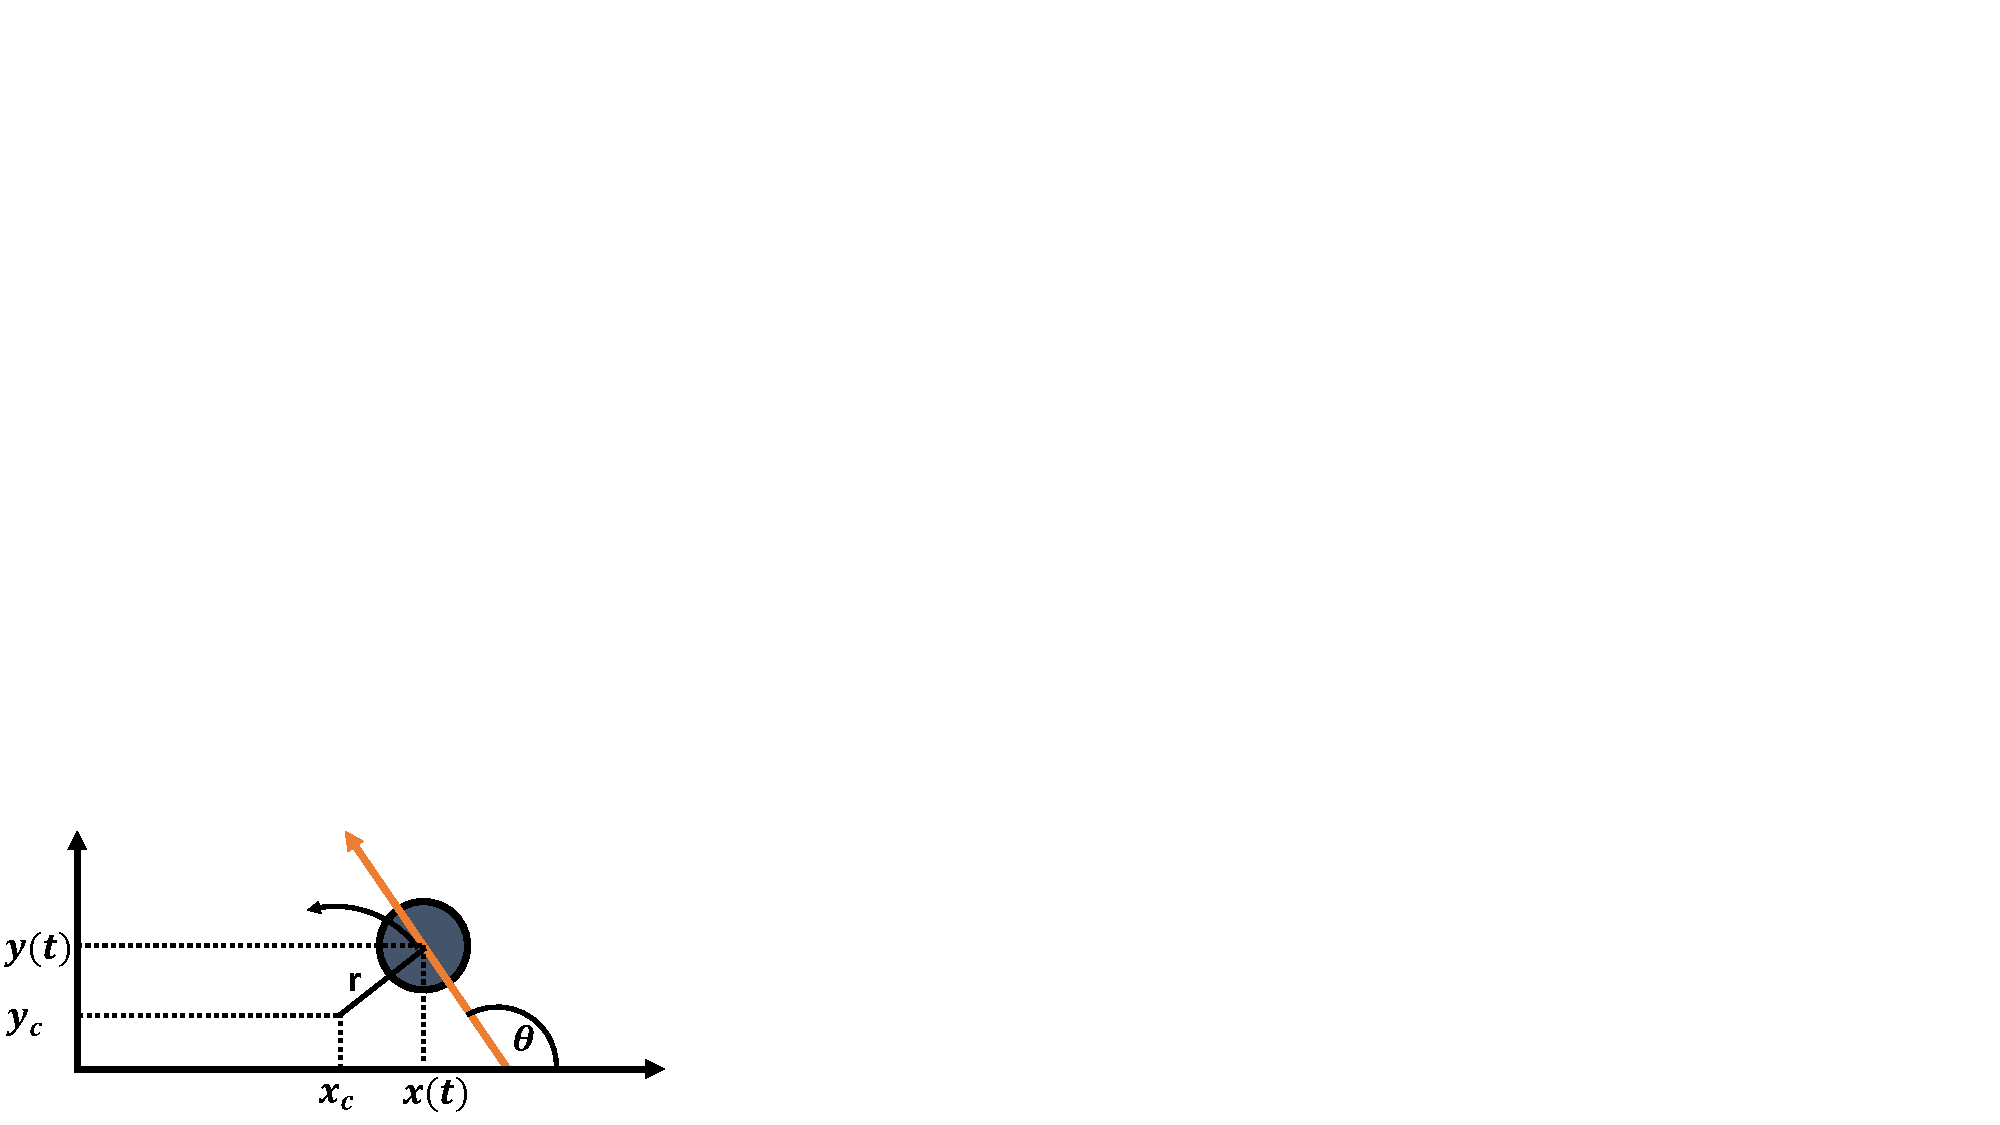
\includegraphics[width=0.6\linewidth, trim={0cm 0cm 24cm 14cm}, clip]{img/Bild_Kinematik_1}
\caption{Darstellung des Momentanpols am Zeitpunkt $t$ \cite[S. 126]{ProbRob}}
\end{figure}

Für den Radius gilt
\begin{equation}
r = \left\vert \frac{v}{\omega}\right\vert\,,
\end{equation}
wobei zu beachten ist, dass der Radius für eine Winkelgeschwindigkeit $\omega=0$ gegen unendlich konvergiert, was wiederum einer reinen Translation entspricht. Aus dem Positionsvektors des Roboters $\mVec{x}_t$ an dem Zeitpunkt $t$ kann der Momentanpol für die folgende Abtastperiode berechnet werden:
\begin{equation}
\label{eq_kinematic_1}
\begin{pmatrix}
x_c \\ y_c
\end{pmatrix} = \begin{pmatrix}
x(t) - \frac{v}{\omega}\cdot \mySin{\theta} \\ y(t) + \frac{v}{\omega}\cdot \myCos{\theta}
\end{pmatrix} \hspace{15pt}\leftrightarrow\hspace{15pt} 
\begin{pmatrix}
x(t) \\ y(t)
\end{pmatrix} = \begin{pmatrix}
x_c + \frac{v}{w}\cdot \mySin{\theta} \\ y_c - \frac{v}{w}\cdot \myCos{\theta}
\end{pmatrix}\,.
\end{equation}
Im nächsten Schritt wird die Bewegung über eine Abtastperiode $\Delta t$ betrachtet, wodurch der Roboter um die Winkeldifferenz $\Delta t\cdot \omega$ auf dem Kreisbogen wandert. Nach \ref{eq_kinematic_1} folgt für den Positionsvektor am Zeitpunkt $t+\Delta t$
\begin{equation}
\label{eq_kinematic_2}
\begin{split}
\begin{pmatrix}
x(t+\Delta t) \\ y(t+\Delta t) \\ \theta(t+\Delta t
\end{pmatrix} &= \begin{pmatrix}
x_c + \frac{v}{w}\cdot \mySin{\theta(t)+\omega\cdot \Delta t} \\ y_c - \frac{v}{w}\cdot \myCos{\theta(t)+\omega \cdot \Delta t} \\ \theta(t) + \omega\cdot \Delta t
\end{pmatrix}\\
& = \begin{pmatrix}
x(t) \\ y(t) \\ \theta(t)
\end{pmatrix} + \begin{pmatrix}
-\frac{v}{\omega}\cdot\mySin{\theta(t)} + \frac{v}{\omega}\cdot \mySin{\theta(t)+\omega \cdot \Delta t} \\
\frac{v}{\omega}\cdot \myCos{\theta(t)} - \frac{v}{w}\cdot \myCos{\theta(t)+\omega \cdot \Delta t}\\
\omega\cdot \Delta t
\end{pmatrix}\,.
\end{split}
\end{equation}
Bisher wurden lediglich deterministische Bewegungen betrachtet. Um nun mögliche Fehler des Steuervektors $\mVec{u}$ zu beachten, werden die störbehafteten Geschwindigkeiten
\begin{equation}
\mVec{u} = \begin{pmatrix}
\hat{v} \\ \hat{\omega}
\end{pmatrix} = \begin{pmatrix}
v + v\idx{err} \\ \omega + \omega\idx{err}
\end{pmatrix}
\end{equation}
eingeführt. Die Zufallsvariablen $v\idx{err}$ und $\omega\idx{err}$ dienen der Fehlermodellierung und ihre Wahrscheinlichkeitsverteilungen $\varepsilon_v$ und $\varepsilon_\omega$ werden dem Anwendungsfall nach angepasst. Einsetzen des stochastischen Steuervektors $\mVec{u}$ liefert
\begin{equation}
\begin{pmatrix}
x(t+\Delta t) \\ y(t+\Delta t) \\ \theta(t+\Delta t
\end{pmatrix} 
=
\begin{pmatrix}
x(t) \\ y(t) \\ \theta(t)
\end{pmatrix} + \begin{pmatrix}
-\frac{\hat{v}}{\hat{\omega}}\cdot\mySin{\theta(t)} + \frac{\hat{v}}{\hat{\omega}}\cdot \mySin{\theta(t)+\hat{\omega} \cdot \Delta t} \\
\frac{\hat{v}}{\hat{\omega}}\cdot \myCos{\theta(t)} - \frac{\hat{v}}{w}\cdot \myCos{\theta(t)+\hat{\omega} \cdot \Delta t}\\
\hat{\omega}\cdot \Delta t
\end{pmatrix}\,.
\end{equation}
In diesem Modell wurden lediglich zwei Zufallsvariablen eingeführt, um die Störung von drei Positionsvariablen zu modellieren. Aus diesem Grund entsteht eine ungewollte stochastische Abhängigkeit zwischen den Elementen des Positionsvektors $\mVec{x}(t+\Delta t)$. Dieses Problem wird behoben, indem eine dritte Zufallsvariable
\begin{equation}
\gamma\idx{err} \equiv \hat{\gamma}
\end{equation}
eingeführt wird, die zu einer zusätzlichen Störung der Orientierung $\theta(t+\Delta t)$ in Form von
\begin{equation}
\label{eq_kinematic_3}
\begin{pmatrix}
x(t+\Delta t) \\ y(t+\Delta t) \\ \theta(t+\Delta t
\end{pmatrix} 
=
\begin{pmatrix}
x(t) \\ y(t) \\ \theta(t)
\end{pmatrix} + \begin{pmatrix}
-\frac{\hat{v}}{\hat{\omega}}\cdot\mySin{\theta(t)} + \frac{\hat{v}}{\hat{\omega}}\cdot \mySin{\theta(t)+\hat{\omega} \cdot \Delta t} \\
\frac{\hat{v}}{\hat{\omega}}\cdot \myCos{\theta(t)} - \frac{\hat{v}}{w}\cdot \myCos{\theta(t)+\hat{\omega} \cdot \Delta t}\\
\hat{\omega}\cdot \Delta t + \hat{\gamma}\cdot \Delta t
\end{pmatrix}
\end{equation}
führt. Die Aufgabe besteht jetzt darin, ein Bewegungsmodell in Form der bedingten Wahrscheinlichkeit
\begin{equation}
\condP{\mVec{x}_t]}{\mVec{u}_t, \mVec{x}_{t-1}}
\end{equation}
zu formulieren. Das heißt es soll eine Funktion aufgestellt werden, die berechnet wie wahrscheinlich der Zustand $\mVec{x}_t$ auf den Zustand $\mVec{x}_{t-1}$ und die Aktion $\mVec{u}_t$ folgt. Dafür wird nach Gleichung (\ref{eq_kinematic_3}) die Werte der stochastisch unabhängigen Zufallsvariablen $v\idx{err}$, $\omega\idx{err}$ und $\gamma\idx{err}$ berechnet. Die gesuchte Wahrscheinlichkeit ergibt sich dann aus deren gemeinsamer Verteilung
\begin{equation}
p(\mVec{x}_t, \mVec{u}_t, \mVec{x}_{t-1}) = \condP{\mVec{x}_t}{\mVec{u}_t, \mVec{x}_{t-1}} = \varepsilon_v(v\idx{err})\cdot \varepsilon_\omega(\omega\idx{err})\cdot \varepsilon_\gamma(\gamma\idx{err})\,.
\end{equation}
Da die direkte Umformung von Gleichung (\ref{eq_kinematic_1}) zur expliziten Darstellung der gesuchten Fehlergrößen zu einem unhandlichen Ergebnis führt, wird eine indirekte Berechnung über den Momentanpol gewählt. Im ersten Schritt werden die Koordinaten des Momentanpols $\mVec{c}$ berechnet, wofür sich nach \cite[S. 130]{ProbRob} \footnote{Schreibweise für $\mVec{x}_t = \begin{pmatrix}
x & y &\theta
\end{pmatrix}^T$, $\mVec{x}_{t+\Delta t} = \begin{pmatrix}
\tilde{x} & \tilde{y} &\tilde{\theta}
\end{pmatrix}^T$}
\begin{equation}
\begin{pmatrix}
x_c \\ y_c
\end{pmatrix} = \begin{pmatrix}
\frac{x+\tilde{x}}{2} + \mu (y-\tilde{y})\\ \frac{y+\tilde{y}}{2}+\mu(\tilde{x}-x)
\end{pmatrix} \hspace{1.5cm}
\mu = \frac{1}{2}\frac{(x-\tilde{x})\myCos{\theta} + (y-\tilde{y})\mySin{\theta}}{(y-\tilde{y})\myCos{\theta}-(x-\tilde{x})\mySin{\theta}}
\end{equation}
ergibt. Woraus sich sowohl der Rotationsradius
\begin{equation}
r\idx{c} = \sqrt{(x-x_c)^2+(y-y_c)^2}
\end{equation}
als auch der auf der Kreisbahn zurückgelegte Winkel 
\begin{equation}
\Delta \theta = \myAtan{\frac{\tilde{y}-y_c}{\tilde{x}-x_c}}-\myAtan{\frac{y-y_c}{x-x_c}}
\end{equation}
berechnen lassen. Mithilfe der der Winkeldifferenz lässt sich wiederum auf die zurückgelegte Strecke
\begin{equation}
\Delta s = r\idx{c}\cdot \Delta \theta
\end{equation}
schließend, welche zusammen auf den gestörten Stellvektor
\begin{equation}
\mVec{\hat{u}} = \begin{pmatrix}
\hat{v}\\ \hat{\omega}
\end{pmatrix} = \frac{1}{\Delta t}\cdot \begin{pmatrix}
\Delta s\\ \Delta \theta
\end{pmatrix}
\end{equation}
führen. Zuletzt fehlt der Orientierungsfehler $\hat{\gamma}$, der sich mithilfe von Gleichung (\ref{eq_kinematic_3}) erschließen lässt.
\begin{equation}
\tilde{\theta}-\theta = \hat{\omega}\cdot \Delta t + \hat{\gamma}\cdot \Delta t
\Leftrightarrow
\hat{\gamma} = \frac{\tilde{\theta}-\theta}{\Delta t} - \hat{\omega}\,.
\end{equation}

\newpage
\section{Messmodell}
Als weiteres Beispiel wird ein stochastisches Messmodell vorgestellt, das später bei der Lokalisierung wiederverwendet wird. Das Ziel des Messmodells ist es den Zusammenhang zwischen einem Zustandsvektor $\mVec{x}\idx{t}$ und einem Messvektor $\mVec{z}\idx{t}$ in Form der bedingten Wahrscheinlichkeit
\begin{equation}
\condP{\mVec{z}\idx{t}}{\mVec{x}\idx{t}}
\end{equation}
herzustellen. Die Verteilung sagt aus, mit welcher Wahrscheinlichkeit ein Messvektor $\mVec{z}\idx{t}$ von einer vorgegebenen Position $\mVec{x}\idx{t}$ aus erzielt wird. Das Messmodell dient als Paradebeispiel dafür, wie heuristische Argumente in stochastische Modelle einfließen können. Unabhängig von dem exakten Sensor wird angenommen, dass es sich um ein auf Messstrahlen basiertes Messprinzip handelt. Das heißt der Messvektor $\mVec{z}\idx{t}$ setzt sich aus mehreren Messwerten $z^k\idx{t}$ zusammen, die jeweils die auf einem Strahl gemessene Distanz wiedergeben. 

Als erste Störgröße wird ein gewöhnliches Messrauschen eingeführt, das als normal verteilt angenommen wird. Der Mittelwert der Verteilung sie die tatsächliche Distanz auf dem Messstrahl, die mit $z^{k*}\idx{t}$ denotiert wird. Als zweiter Parameter muss die Varianz $\sigma\idx{hit}$ festgelegt werden, die angibt wie stark der Messwert von dem Rauschen beeinflusst wird. Somit ergibt sich als Modell für das Sensorrauschen
\begin{equation}
p\idx{hit}\left( z^{k}\idx{t} \mCond \mVec{x}\idx{t} \right) = \left\{ \begin{array}{cl}
\eta \cdot \mathcal{N}(z^k\idx{t}, z^{k*}\idx{t}, \sigma^2\idx{hit}) & \hspace{5mm}\forall z^k\idx{t} \in \left[0, z\idx{max}\right] \\
0 & \hspace{5mm} \forall z^k\idx{t} \notin \left[0, z\idx{max}\right]
\end{array}\right. \,.
\end{equation}
Die Messwerte werden außerdem von unerwarteten Objekten beeinflusst. Angenommen es liegt eine Karte der Umgebung vor und es bewegt sich ein Mensch innerhalb des Raumes. Wenn der Mensch nun die Messstrahlen unterbricht tritt ein geringerer Messwert als anhand der Karte erwartet ein. Im Allgemeinen gilt, dass im Falle von Störungen durch unerwartete Objekte die Messwerte lediglich kleiner, aber niemals größer werden. Des Weiteren nimmt die Wahrscheinlichkeit, dass ein Messwert von einem Objekt beeinflusst wird mit zunehmendem Messdistanz ab. Für das Modell wird eine exponentiell abfallende Verteilung
\begin{equation}
\renewcommand*{\arraystretch}{1.3}
p\idx{short}\left( z^k\idx{t} \mCond \mVec{x}\idx{t} \right) = \left\{ \begin{array}{cl}
\eta \cdot \lambda\idx{short}\cdot e^{-\lambda\idx{short}\cdot z^{k}\idx{t}} & \hspace{5mm} \forall z^{k}\idx{t} \in \left[0, z^{k*}\idx{t}\right] \\
0 & \hspace{5mm} \forall z^{k}\idx{t} \notin \left[0, z^{k*}\idx{t}\right]
\end{array}\right. 
\end{equation}
gewählt, wobei $\lambda\idx{short}$ als wählbarer Parameter die Häufigkeit der Störungen widerspiegelt.

Als dritte Ursache für Messfehler wird das sporadische Versagen des Sensors herangezogen. Derartige Phänomene können bei Laserscannern auftreten, wenn beispielsweise schwarze Oberflächen die Strahlen vollständig absorbieren. Ähnliche Probleme werden bei Sonarsensoren durch Interferenz oder schallabsorbierende Medien hervorgerufen. Unabhängig von dem Messprinzip des Sensors werden in all den beschriebenen Fällen - fälschlicherweise - maximale Distanzen gemessen, wodurch die Verteilung
\begin{equation}
p\idx{max}\left(z^k\idx{t} \mCond \mVec{x}\idx{t}\right) = \left\{ \begin{array}{cl}
1 & \hspace{5mm} \forall z = z\idx{max} \\
0 & \hspace{5mm} \forall z  \neq z\idx{max}
\end{array}\right.
\end{equation}
motiviert wird. {\color{red} Die Aussage von dieser Verteilung ist ein bisschen Banane, wenn wenn der Messwert den maximal Möglichen anzeigt, ist die dass 100 Prozent der Fall, ansonsten nicht? Oder ist es so zu verstehen, dass ein maximaler Messwert zu 100 Prozent den Fall von Messfehler bedeutet? Dann müsste ich die Interpretation der anderen Verteilungen nochmal überdenken}

Als letzter und absurdester Fall werden rein zufällig falsche Phänomene betrachtet. Als Argument dient die Beobachtung, dass es unerklärliche Messwerte gibt, die - zu Gunsten der Simplizität - durch eine Gleichverteilung der Form
\begin{equation}
\renewcommand*{\arraystretch}{1.3}
p\idx{rand}\left( z^k\idx{t} \mCond \mVec{x}\idx{t}\right) = \left\{ \begin{array}{cl}
\frac{1}{z\idx{max}} & \hspace{5mm} \forall z^k\idx{t} \in \left[0, z\idx{max}\right] 
\\
0 & \hspace{5mm} \forall z^k\idx{t} \notin \left[0, z\idx{max}\right]
\end{array} \right.
\end{equation}
repräsentiert werden. Es liegt schließlich nahe das komplexeste aller Probleme durch die simpelste aller Darstellung zu beschreiben. An diesem Beispiel wird deutlich, dass heuristische Einflüsse in stochastischen Modellen auch mit variierendem Elan verteidigt werden.

Die gesuchte Wahrscheinlichkeit $\condP{z^k\idx{t}}{\mVec{x}\idx{t}}$ wird aus Summe der vier Verteilung berechnet, wobei diese mit den Faktoren $z\idx{hit}$, $z\idx{short}$, $z\idx{max}$ und $z\idx{rand}$ gewichtet werden. Die Gewichtung erlauben es dem Anwender, die Heuristiken nach ihrer Glaubhaftigkeit zu bewerten.
\begin{equation}
\condP{z^k\idx{t}}{\mVec{x}\idx{t}} = \begin{bmatrix} z\idx{hit} & z\idx{short} & z\idx{max} z\idx{rand} \end{bmatrix} \cdot \begin{bmatrix}
p\idx{hit}\left( z^{k}\idx{t} \mCond \mVec{x}\idx{t} \right) \\
p\idx{short}\left( z^k\idx{t} \mCond \mVec{x}\idx{t} \right) \\
p\idx{max}\left(z^k\idx{t} \mCond \mVec{x}\idx{t}\right) \\
p\idx{rand}\left( z^k\idx{t} \mCond \mVec{x}\idx{t}\right)
\end{bmatrix}\,.
\end{equation}
